\subsection{UGV01 August 29 AprilTag Validation Update}
\label{subsec:ugv01-aug29-validation}

To tighten the UGV01 asset-specific instantiation evidence, we processed a new
overhead AprilTag recording captured on August 29, 2026 together with the
matching direct telemetry log. The recording used a $2.0\,\text{m}\times
1.0\,\text{m}$ rectangular world layout with fixed tags $1$--$4$ and rover tag
$0$. The best paired run was
\texttt{WIN\_20260829\_15\_35\_55\_Pro.mp4} with matching telemetry
\texttt{WIN\_20260829\_15\_35\_55\_Pro\_telemetry\_adapted.csv}. The AprilTag
tracking itself was clean: all five tags were decoded in all $4990/4990$ video
frames, and the approximately $10$ Hz fidelity evaluation retained $1664$
directly decoded samples with no temporally recovered segments.

We first evaluated the current UGV01 baseline setting, then ran a same-session
temporal calibration on the first $75\%$ of the recording and re-evaluated the
full run with the fitted parameters. The baseline used the current development
candidate already stored in the repository:
distance scale $0.975$, clockwise effective track width $0.200\,\text{m}$,
counterclockwise effective track width $0.190\,\text{m}$, and gyro blend weight
$0.20$. The temporal calibration selected a more aggressive asymmetric turn
model with distance scale $0.95$, clockwise width $0.17\,\text{m}$,
counterclockwise width $0.28\,\text{m}$, and the same gyro weight.

The full-window fitted result materially improved translational fidelity. The
position ATE RMSE dropped from $0.410\,\text{m}$ to $0.198\,\text{m}$, the
median position error dropped from $0.297\,\text{m}$ to $0.178\,\text{m}$, and
the position p95 dropped from $0.860\,\text{m}$ to $0.321\,\text{m}$.
Short-horizon local fidelity improved as well: $1$ s RPE RMSE decreased from
$0.0509\,\text{m}$ to $0.0241\,\text{m}$. Heading agreement also improved, with
heading MAE decreasing from $76.6^\circ$ to $48.6^\circ$, but this component
remains the weakest part of the current run and is not yet strong enough to be
treated as final publication-grade heading validation.

The synchronization estimate was stable enough for a meaningful pilot
comparison, but it still relied on motion correlation rather than a deliberate
hardware-visible synchronization event. The fitted run used an estimated
video-minus-telemetry offset of approximately $-2.00\,\text{s}$ with
synchronization uncertainty up to $0.23\,\text{s}$. The fitted run also
improved synchronization activity correlation from $0.870$ to $0.884$. Camera
stationary jitter was negligible in this clip
($3.25\times 10^{-5}\,\text{m}$ RMSE), so the dominant remaining uncertainty is
not raw image noise but rather heading drift, path-length inflation, and the
absence of a hard synchronization pulse.

Figure~\ref{fig:ugv01-aug29-summary} summarizes the same-run full-window gains
and the temporal-tail diagnostic. Figure~\ref{fig:ugv01-aug29-trajectory}
shows the fitted physical-versus-virtual trajectory comparison, and
Figure~\ref{fig:ugv01-aug29-diagnostics} shows the detailed fidelity traces.
Taken together, these results strengthen the UGV01 instantiation story in an
important but still bounded way: the new August 29 run demonstrates that the
current twin can be materially tightened on real rover data, especially for
position and short-horizon motion, but it also shows that heading fidelity and
strict synchronization still need one final clean paired run before the UGV01
section is fully frozen.

\begin{figure}[t]
    \centering
    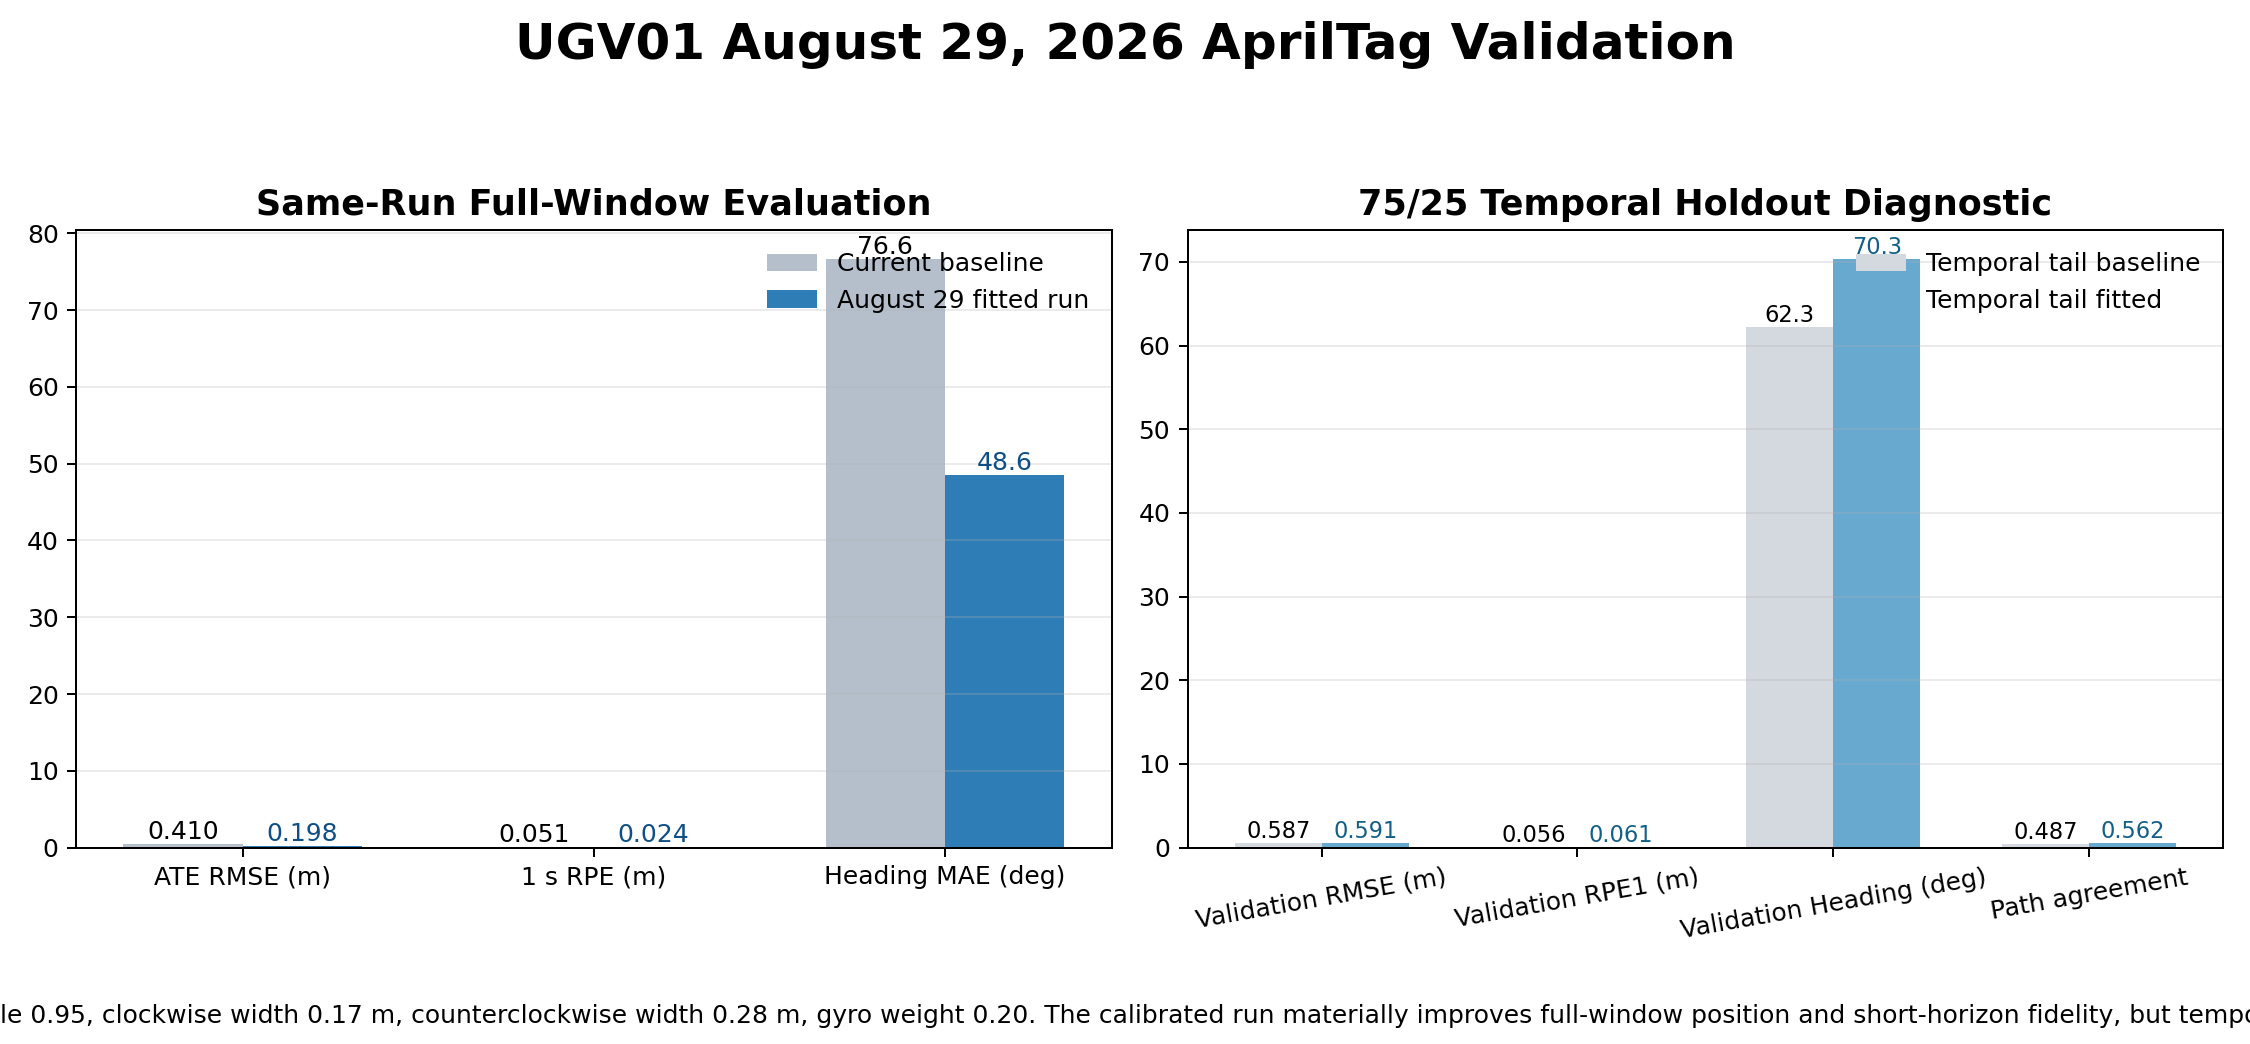
\includegraphics[width=\linewidth]{figures/ugv01_aug29_validation_summary.png}
    \caption{August 29, 2026 UGV01 AprilTag validation summary. The same-run
    fitted model substantially improves full-window position ATE and $1$ s RPE
    relative to the current baseline. The $75/25$ temporal holdout diagnostic
    shows that these gains do not yet transfer cleanly to the held-out tail,
    especially for heading.}
    \label{fig:ugv01-aug29-summary}
\end{figure}

\begin{figure}[t]
    \centering
    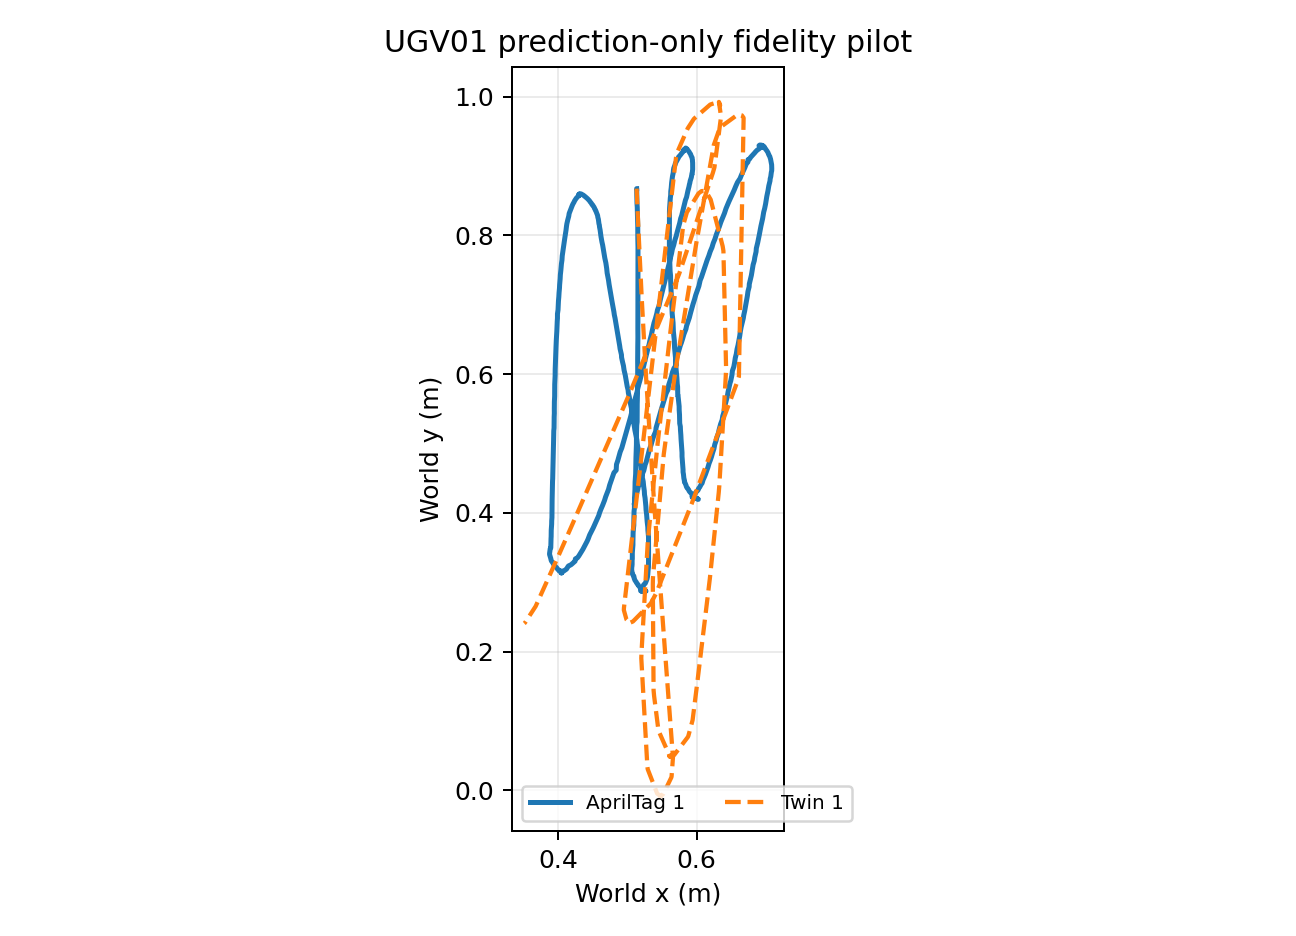
\includegraphics[width=\linewidth]{figures/ugv01_aug29_trajectory_fidelity.png}
    \caption{Trajectory comparison for the fitted August 29 UGV01 run against
    the AprilTag physical reference. The fitted model tracks the local route
    shape more closely than the current baseline and reduces the global
    translational disagreement over the full run.}
    \label{fig:ugv01-aug29-trajectory}
\end{figure}

\begin{figure}[t]
    \centering
    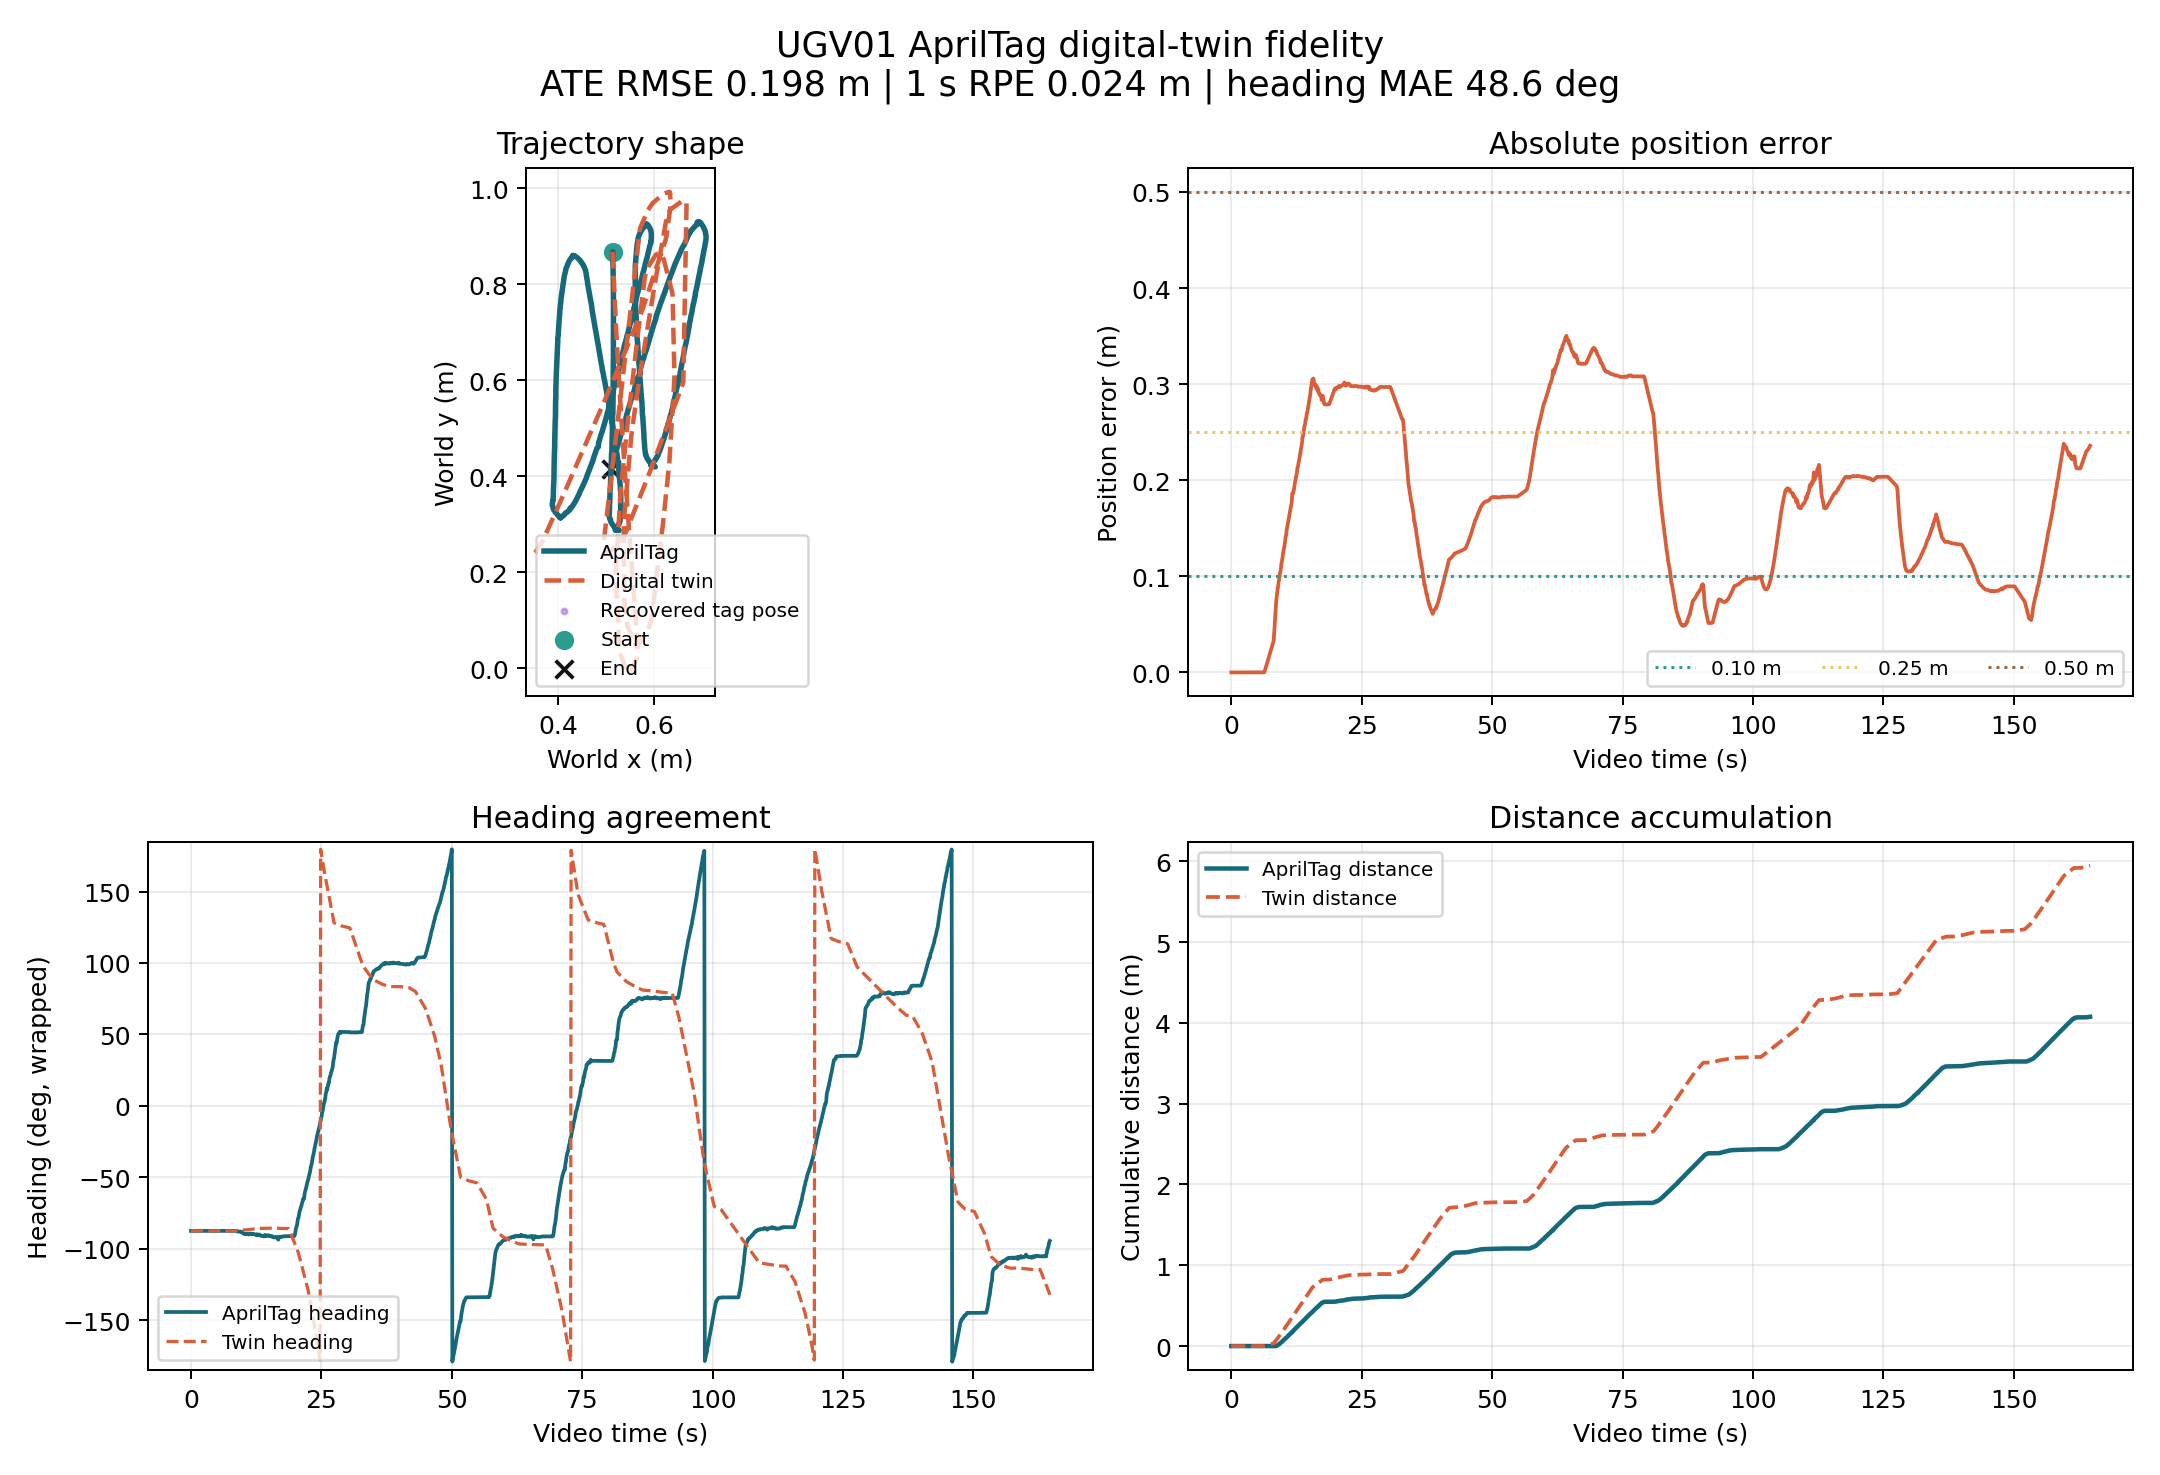
\includegraphics[width=\linewidth]{figures/ugv01_aug29_fidelity_diagnostics.png}
    \caption{Detailed diagnostics for the fitted August 29 UGV01 validation
    run. Position error improves materially, but the heading traces still show
    accumulated disagreement, which is why this run should be treated as a
    strong pilot update rather than the final frozen UGV01 heading result.}
    \label{fig:ugv01-aug29-diagnostics}
\end{figure}
